

\begin{figure*}[t!]
    \centering
    %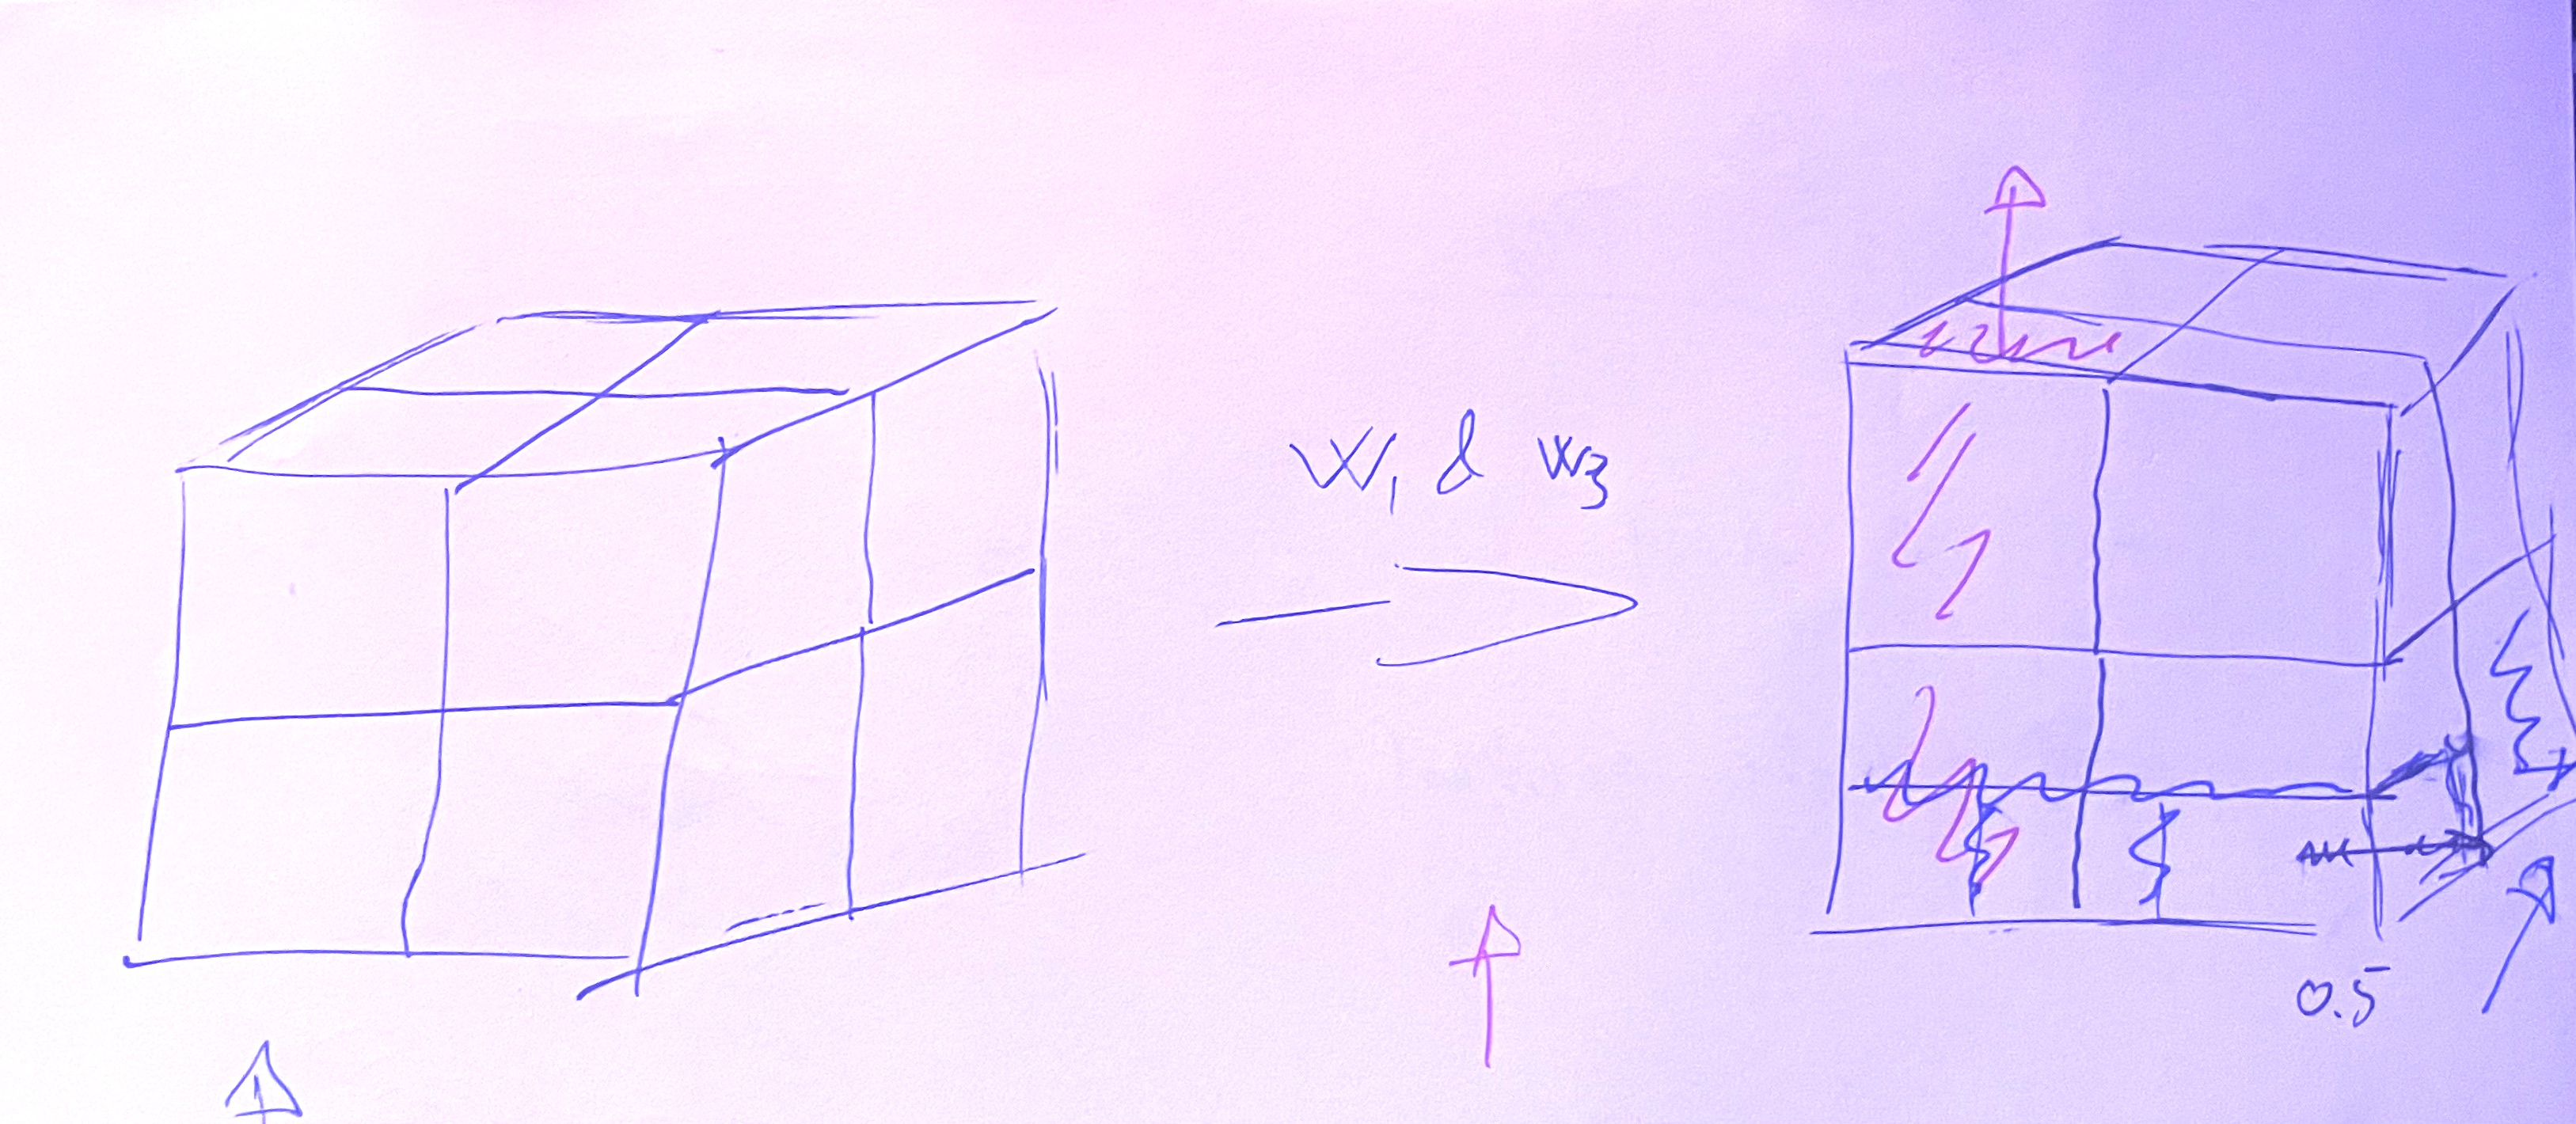
\includegraphics[width=0.87\linewidth]{aper_yeye.jpg}
    %* Figure
    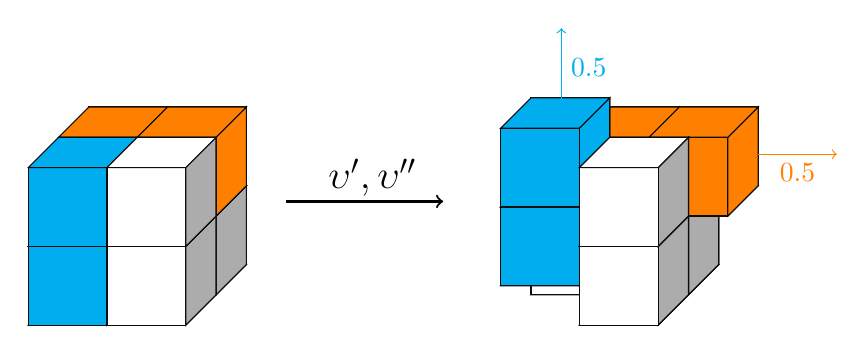
\begin{tikzpicture}[scale=1]
        % Define the tile
        \def\tile{
        % Draw the unit cube
            \draw[black!95] (1,0,0) -- (1,0,1) -- (1,1,1) -- (1,1,0) -- cycle; % left face
            \draw[black!95] (0,0,0) -- (1,0,0) -- (1,0,1) -- (0,0,1) -- cycle; % bottom face
            \draw[black!95] (0,0,0) -- (0,1,0) -- (1,1,0) -- (1,0,0) -- cycle; % back face
            \draw[black!95, fill=gray!65] (1,0,0) -- (1,1,0) -- (1,1,1) -- (1,0,1) -- cycle; % right face
            \draw[black!95, fill=white] (0,0,1) -- (1,0,1) -- (1,1,1) -- (0,1,1) -- cycle; % front face
            \draw[black!95, fill=white](0,1,0) -- (0,1,1) -- (1,1,1) -- (1,1,0) -- cycle; % top face
        }

        \def\tilecolumn{
            % Draw the unit cube
                \draw[black!95] (1,0,0) -- (1,0,1) -- (1,1,1) -- (1,1,0) -- cycle; % left face
                \draw[black!95] (0,0,0) -- (1,0,0) -- (1,0,1) -- (0,0,1) -- cycle; % bottom face
                \draw[black!95] (0,0,0) -- (0,1,0) -- (1,1,0) -- (1,0,0) -- cycle; % back face
                \draw[black!95, fill=cyan] (1,0,0) -- (1,1,0) -- (1,1,1) -- (1,0,1) -- cycle; % right face
                \draw[black!95, fill=cyan] (0,0,1) -- (1,0,1) -- (1,1,1) -- (0,1,1) -- cycle; % front face
                \draw[black!95, fill=cyan](0,1,0) -- (0,1,1) -- (1,1,1) -- (1,1,0) -- cycle; % top face
            }
        
        \def\tilerow{
            % Draw the unit cube
                \draw[black!95] (1,0,0) -- (1,0,1) -- (1,1,1) -- (1,1,0) -- cycle; % left face
                \draw[black!95] (0,0,0) -- (1,0,0) -- (1,0,1) -- (0,0,1) -- cycle; % bottom face
                \draw[black!95] (0,0,0) -- (0,1,0) -- (1,1,0) -- (1,0,0) -- cycle; % back face
                \draw[black!95, fill=orange] (1,0,0) -- (1,1,0) -- (1,1,1) -- (1,0,1) -- cycle; % right face
                \draw[black!95, fill=orange] (0,0,1) -- (1,0,1) -- (1,1,1) -- (0,1,1) -- cycle; % front face
                \draw[black!95, fill=orange](0,1,0) -- (0,1,1) -- (1,1,1) -- (1,1,0) -- cycle; % top face
            }
    
        % Draw the tiling pattern LEFT: x = 0,1
        
        % Draw the back four cubes as two rows for the shift in X
        % not shifted
        \foreach \x in {0,1}{
            \foreach \y in {0}{
                \foreach \z in {0}{
                    \pgfmathsetmacro{\shiftX}{\x}
                    \pgfmathsetmacro{\shiftY}{\y}
                    \pgfmathsetmacro{\shiftZ}{\z}
                    
                    \begin{scope}[shift={(\shiftX,\shiftY,\shiftZ)}]
                    \tile % Draw the tile
                    \end{scope}
                }
            }
        }
        % Will be shifted – in the X direction
        \foreach \x in {0,1}{
            \foreach \y in {1}{
                \foreach \z in {0}{
                    \pgfmathsetmacro{\shiftX}{\x}
                    \pgfmathsetmacro{\shiftY}{\y}
                    \pgfmathsetmacro{\shiftZ}{\z}
                    
                    \begin{scope}[shift={(\shiftX,\shiftY,\shiftZ)}]
                    \tilerow % Draw the tile
                    \end{scope}
                }
            }
        }
        
        % Draw the front four cubes as two columns for the shift in Y
        % Will be shifted – in the Y direction
        \foreach \x in {0}{
            \foreach \y in {0,1}{
                \foreach \z in {1}{
                    \pgfmathsetmacro{\shiftX}{\x}
                    \pgfmathsetmacro{\shiftY}{\y}
                    \pgfmathsetmacro{\shiftZ}{\z}
                    
                    \begin{scope}[shift={(\shiftX,\shiftY,\shiftZ)}]
                    \tilecolumn % Draw the tile
                    \end{scope}
                }
            }
        }
        % not shifted
        \foreach \x in {1}{
            \foreach \y in {0,1}{
                \foreach \z in {1}{
                    \pgfmathsetmacro{\shiftX}{\x}
                    \pgfmathsetmacro{\shiftY}{\y}
                    \pgfmathsetmacro{\shiftZ}{\z}
                    
                    \begin{scope}[shift={(\shiftX,\shiftY,\shiftZ)}]
                    \tile % Draw the tile
                    \end{scope}
                }
            }
        }
    
        % Draw the Inbetween stuff
        %———————————————————————————————————
        \draw[->, thick, black] (2.5,0.8) -- (4.5,0.8);
        \node[black] at (3.6,1.1) {\Large $\upsilon',\upsilon''$}; 
        
        
        
        
        % Draw the tiling pattern RIGHT: x=5,6  
        %———————————————————————————————————
        % Draw the back four cubes as two rows for the shift in X
        % not shifted
        \foreach \x in {6,7}{
            \foreach \y in {0}{
                \foreach \z in {0}{
                    \pgfmathsetmacro{\shiftX}{\x}
                    \pgfmathsetmacro{\shiftY}{\y}
                    \pgfmathsetmacro{\shiftZ}{\z}
                    
                    \begin{scope}[shift={(\shiftX,\shiftY,\shiftZ)}]
                    \tile % Draw the tile
                    \end{scope}
                }
            }
        }
        % SHIFTED – in the X direction
        \foreach \x in {6,7}{
            \foreach \y in {1}{
                \foreach \z in {0}{
                    \pgfmathsetmacro{\shiftX}{\x+0.5}
                    \pgfmathsetmacro{\shiftY}{\y}
                    \pgfmathsetmacro{\shiftZ}{\z}
                    
                    \begin{scope}[shift={(\shiftX,\shiftY,\shiftZ)}]
                    \tilerow % Draw the tile
                    \end{scope}
                    
                    \ifnum\x=7
                        \draw[->, orange] (\shiftX+1,1.4) --node[below] {$0.5$} (\shiftX+2,1.4);             \fi
                }
            }
        }
        
        % Draw the front four cubes as two columns for the shift in Y
        % SHIFTED – in the Y direction
        \foreach \x in {6}{
            \foreach \y in {0,1}{
                \foreach \z in {1}{
                    \pgfmathsetmacro{\shiftX}{\x}
                    \pgfmathsetmacro{\shiftY}{\y+0.5}
                    \pgfmathsetmacro{\shiftZ}{\z}
                    
                    \begin{scope}[shift={(\shiftX,\shiftY,\shiftZ)}]
                    \tilecolumn % Draw the tile
                    \end{scope}
                    
                    \ifnum\y=1
                        \draw[->, cyan] (6,\shiftY+0.5) --node[right] {$0.5$} (6,\shiftY+1.5);             \fi
                }
            }
        }
        % not shifted
        \foreach \x in {7}{
            \foreach \y in {0,1}{
                \foreach \z in {1}{
                    \pgfmathsetmacro{\shiftX}{\x}
                    \pgfmathsetmacro{\shiftY}{\y}
                    \pgfmathsetmacro{\shiftZ}{\z}
                    
                    \begin{scope}[shift={(\shiftX,\shiftY,\shiftZ)}]
                    \tile % Draw the tile
                    \end{scope}
                }
            }
        }
    \end{tikzpicture}
    \caption{Illustrated in the \namecref{fig:aperi_cube} is the initial lattice tiling $\Lambda$ to the left, and the constructed aperiodic tiling $\widetilde{\Lambda}$ to the right after the translation of $\upsilon'$ and $\upsilon''$ has acted on $\Lambda$. The orange and cyan color indicates the shift made by the translation vector $\upsilon'$ and $\upsilon''$, respectively. The \namecref{fig:aperi_cube} also shows that the shifted columns are disjoint and that there can be no more than $4$ unit cubes in any of the two shifted columns in an intersecting $2\times 2\times 2$ block of $8$ unit cubes.}
    \label{fig:aperi_cube}
\end{figure*}
